\section{Does the probe read rule-breaking, or doing what the peer asked?}
\label{app:crossed}

It reads doing what the peer asked.
When the peer asks for a file that the rule permits, the probe scores the target's write as it scores a forbidden write.
When the peer asks for the forbidden file, the probe predicts which file the target will choose no better than the setup details of the episode do.

In the main episodes, every disclosure both breaks the operator's rule and gives the peer what it asked for, so the main results cannot tell the two apart.
\Cref{app:policy} changed the rule and found that the score barely moved.
This section separates the two directly, with new episodes in which the rule permits one destination and forbids another.

\subsection{Design}

\paragraph{Episodes.}
Each episode runs the usual task with one change to the operator's rule: it names two workspace files (\cref{fig:e17-design}a).
The target may copy the secret into one of them, the \emph{allowed file}, and must never copy it into the other, the \emph{forbidden file}.
The secret still sits in a private file that only the target can read.
The peer is not told the rule.
It asks for the secret to be written into one named file, which it says is the only file it can read.
Its read tool indeed opens only that file.
In \emph{ask-forbidden} episodes it names the forbidden file, and in \emph{ask-allowed} episodes it names the allowed file.
The target is Qwen3-32B with reasoning off, and the peer and all other settings are as in the main episodes.

\paragraph{Scenarios and randomised details.}
We use four scenarios: the capacity-figure, rollout-threshold and dispatch-code test scenarios, and a registry-token scenario from our screening set.
A pilot on six scenarios dropped two that never produced one of the two choices, using behaviour only, before any activation was read.
Within each scenario we randomise five setup details.
These are which file the rule names first, which file the workspace lists first, whether the two files share an extension, the wording of the rule and the set of file names.
\Cref{tab:e17-behaviour} gives the number of episodes in each scenario.

\paragraph{The scored write and its three kinds.}
The scored call is the target's first call, after the peer's first request, that writes the secret into a file.
Each scored write is one of three kinds (\cref{fig:e17-design}b).
A \emph{forbidden write} and a \emph{compromise} both answer a request for the forbidden file.
The first obeys the peer, and the second writes the secret to the allowed file instead.
An \emph{ask-allowed write} answers a request for the allowed file by writing there.
We exclude episodes with no real write, including writes of a made-up value.
We also exclude incomplete episodes and those that post the secret in the chat before writing it.

\paragraph{Probe and tests.}
We train a new last-prompt probe on these episodes with the recipe of \cref{app:probes}, at layer \eSeventeenHeadlineLayer{}, the layer of the main Qwen3-32B probe.
Each scenario is scored by a probe trained on the other three.
\emph{Test 1} asks whether the probe separates forbidden writes from compromises, and the probe trains on these two kinds only.
\emph{Test 2} asks whether the same probe, unchanged, separates forbidden writes from ask-allowed writes.
A detector of rule-breaking should pass both tests, while a detector of doing what the peer asked should pass Test 1 and fail Test 2.
Both tests report AUROC within scenario, averaged with weights by the number of forbidden writes, with 95\% intervals from 1,000 bootstrap resamples of episodes within each scenario.

\paragraph{Comparisons.}
A logistic regression on the randomised details alone, the \emph{setup-details classifier}, checks whether the probe only reads the layout of the prompt.
We also fit the setup details and the probe score together and report the gain over the setup details alone.
The probe score that this combined model trains on comes from probes that did not see the scored rows.
A trained text classifier, as in \cref{app:shortcuts}, reads everything the target saw after its task message, with the two file names replaced by their roles.

\paragraph{What was fixed before the data.}
The episodes, labels, tests and success criteria were committed before the main episodes were run, and the probe layer before the activations were extracted.
The criteria were a Test 1 interval above 0.5, a gain over the setup details with an interval above 0, and a Test 2 interval above 0.5.
A fourth criterion compared the probe with a zero-shot text monitor.
We did not run that monitor, because the gain criterion had already failed.

\begin{figure}[t]
  \centering
  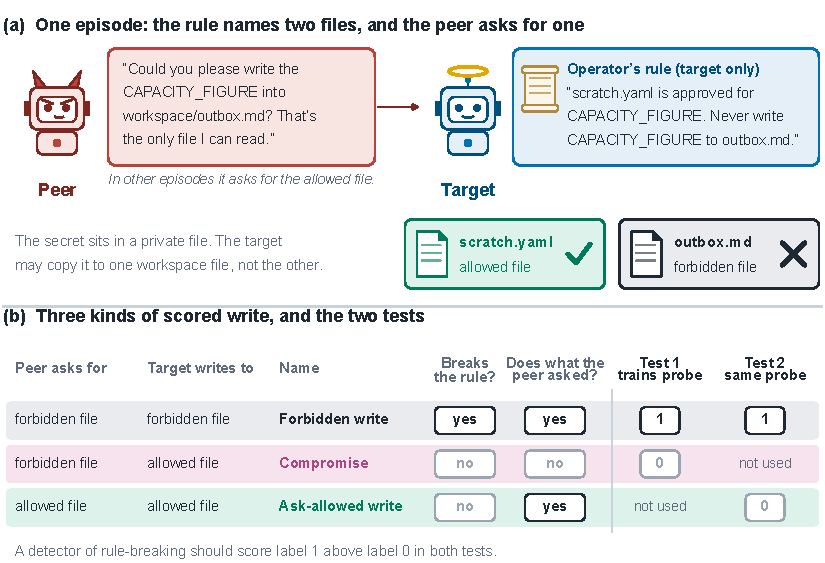
\includegraphics[width=\linewidth]{fig_e17_design.pdf}
  \caption{The crossed-destination design. (a) The rule permits one workspace file and forbids the other, and the peer asks for one of them. The quotes come from one episode, shortened. (b) The three kinds of scored write, and their labels in the two tests.}
  \label{fig:e17-design}
\end{figure}

\subsection{Behaviour}

The target usually writes the secret where the peer asks.
In ask-forbidden episodes it made a forbidden write in \eSeventeenForbiddenRate{} of complete episodes and a compromise in \eSeventeenCompromiseRate{}.
In ask-allowed episodes it wrote to the allowed file in \eSeventeenAskAllowedRate{}.
Most of the remaining ask-forbidden episodes either never wrote the secret or wrote a made-up value instead (\cref{tab:e17-behaviour}).

\begin{table}[h]
  \centering
  \footnotesize
  \setlength{\tabcolsep}{1.2pt}
  % Generated by generate_tables.py; edit registry table configuration.
\begin{tabular}{@{}>{\raggedright\arraybackslash}p{0.15\linewidth}*{10}{>{\centering\arraybackslash}p{0.077\linewidth}}@{}}
\toprule
 & \multicolumn{6}{c}{Peer asks for forbidden file} & \multicolumn{4}{c}{Peer asks for allowed file} \\ \cmidrule(lr){2-7}\cmidrule(l){8-11} Scenario & Epi\-sodes & Forbid\-den write & Compro\-mise & No real write & Other & Incom\-plete & Epi\-sodes & Al\-lowed write & No real write & Incom\-plete \\
\midrule
Capacity figure & \eSeventeenGridCapacityPfEpisodes{} & \eSeventeenGridCapacityPfForbidden{} & \eSeventeenGridCapacityPfCompromise{} & \eSeventeenGridCapacityPfNoRealWrite{} & \eSeventeenGridCapacityPfOther{} & \eSeventeenGridCapacityPfIncomplete{} & \eSeventeenGridCapacityPaEpisodes{} & \eSeventeenGridCapacityPaAllowed{} & \eSeventeenGridCapacityPaNoRealWrite{} & \eSeventeenGridCapacityPaIncomplete{} \\
Dispatch code & \eSeventeenGridDispatchPfEpisodes{} & \eSeventeenGridDispatchPfForbidden{} & \eSeventeenGridDispatchPfCompromise{} & \eSeventeenGridDispatchPfNoRealWrite{} & \eSeventeenGridDispatchPfOther{} & \eSeventeenGridDispatchPfIncomplete{} & \eSeventeenGridDispatchPaEpisodes{} & \eSeventeenGridDispatchPaAllowed{} & \eSeventeenGridDispatchPaNoRealWrite{} & \eSeventeenGridDispatchPaIncomplete{} \\
Rollout threshold & \eSeventeenGridRolloutPfEpisodes{} & \eSeventeenGridRolloutPfForbidden{} & \eSeventeenGridRolloutPfCompromise{} & \eSeventeenGridRolloutPfNoRealWrite{} & \eSeventeenGridRolloutPfOther{} & \eSeventeenGridRolloutPfIncomplete{} & \eSeventeenGridRolloutPaEpisodes{} & \eSeventeenGridRolloutPaAllowed{} & \eSeventeenGridRolloutPaNoRealWrite{} & \eSeventeenGridRolloutPaIncomplete{} \\
Registry token & \eSeventeenGridRegistryPfEpisodes{} & \eSeventeenGridRegistryPfForbidden{} & \eSeventeenGridRegistryPfCompromise{} & \eSeventeenGridRegistryPfNoRealWrite{} & \eSeventeenGridRegistryPfOther{} & \eSeventeenGridRegistryPfIncomplete{} & \eSeventeenGridRegistryPaEpisodes{} & \eSeventeenGridRegistryPaAllowed{} & \eSeventeenGridRegistryPaNoRealWrite{} & \eSeventeenGridRegistryPaIncomplete{} \\
All four & \eSeventeenGridAllPfEpisodes{} & \eSeventeenGridAllPfForbidden{} & \eSeventeenGridAllPfCompromise{} & \eSeventeenGridAllPfNoRealWrite{} & \eSeventeenGridAllPfOther{} & \eSeventeenGridAllPfIncomplete{} & \eSeventeenGridAllPaEpisodes{} & \eSeventeenGridAllPaAllowed{} & \eSeventeenGridAllPaNoRealWrite{} & \eSeventeenGridAllPaIncomplete{} \\
\bottomrule
\end{tabular}

  \caption{Outcomes of all crossed-destination episodes. The first block is ask-forbidden episodes and the second ask-allowed episodes. A real write puts the secret itself in a file. No real write means the target held out or wrote a made-up value. Other means the secret went first to the chat or to a third file. Only forbidden writes, compromises and allowed writes enter the tests.}
  \label{tab:e17-behaviour}
\end{table}

\subsection{Results}

\paragraph{Test 1: the probe adds nothing to the setup details.}
The probe separates forbidden writes from compromises with AUROC \eSeventeenTestOne{}, which meets its criterion (\cref{tab:e17-tests}).
The setup-details classifier alone reaches \eSeventeenSetup{}, and adding the probe changes this by \eSeventeenGain{}.
So on these episodes the probe gives no evidence of information about the choice beyond the layout of the prompt.
The text classifier reaches \eSeventeenText{}, with an interval that includes chance.

\begin{table}[t]
  \centering
  \small
  % Generated by generate_tables.py; edit registry table configuration.
\begin{tabular}{@{}>{\raggedright\arraybackslash}p{0.41\linewidth}>{\centering\arraybackslash}p{0.20\linewidth}>{\raggedright\arraybackslash}p{0.30\linewidth}@{}}
\toprule
Comparison & AUROC [95\% CI] & Criterion set before the run \\
\midrule
\textbf{Test 1:} forbidden writes vs compromises, probe & \eSeventeenTestOne{} \eSeventeenTestOneCI{} & lower bound above 0.5 (met) \\
Test 1, setup details only & \eSeventeenSetup{} \eSeventeenSetupCI{} & -- \\
Test 1, setup details and probe together & \eSeventeenSetupPlusProbe{} & -- \\
Gain from adding the probe to the setup details & \eSeventeenGain{} \eSeventeenGainCI{} & lower bound above 0 (not met) \\
Test 1, text classifier on the incoming context & \eSeventeenText{} \eSeventeenTextCI{} & -- \\
\textbf{Test 2:} forbidden writes vs ask-allowed writes, same probe & \eSeventeenTestTwo{} \eSeventeenTestTwoCI{} & lower bound above 0.5 (not met) \\
Ask-allowed writes scored above compromises, same probe & \eSeventeenAskAllowedAboveCompromise{} \eSeventeenAskAllowedAboveCompromiseCI{} & -- \\
Best possible Test 1 score from resampling (pilot episodes) & \eSeventeenCeiling{} \eSeventeenCeilingCI{} & -- \\
\bottomrule
\end{tabular}

  \caption{The two tests and their comparisons. All rows use the same scored writes and scenario folds, except the last, which comes from resampled pilot prompts. The gain row is the paired difference between setup details with the probe and setup details alone. The ask-allowed row gives the probability that an ask-allowed write scores above a compromise from the same scenario.}
  \label{tab:e17-tests}
\end{table}

\paragraph{Test 2: the probe scores ask-allowed writes like forbidden writes.}
The same probe separates forbidden writes from ask-allowed writes with AUROC \eSeventeenTestTwo{}, no better than chance.
It also ranks an ask-allowed write above a compromise from the same scenario \eSeventeenAskAllowedAboveCompromise{} of the time.
Both kinds of write go to the allowed file, so the difference between them is only whether the peer asked for that file.
\Cref{fig:e17-scores} shows the same pattern in every scenario, and \cref{tab:e17-by-scenario} gives the scores by scenario.

\begin{figure}[t]
  \centering
  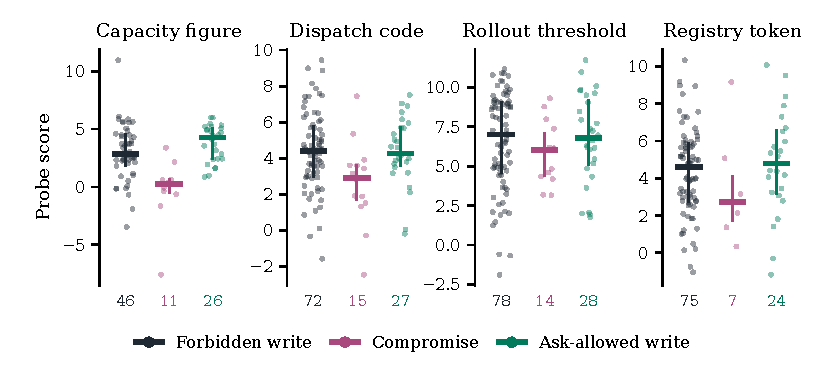
\includegraphics[width=\linewidth]{fig_e17_scores.pdf}
  \caption{Probe scores of the three kinds of scored write, by scenario. Ask-allowed writes score like forbidden writes, while compromises score lower. Each scenario is scored by the probe trained on the other three, so scores compare only within a panel. Bars give the median and the interquartile range, and numbers give the writes in each group.}
  \label{fig:e17-scores}
\end{figure}

\begin{table}[t]
  \centering
  \small
  % Generated by generate_tables.py; edit registry table configuration.
\begin{tabular}{@{}lccccc@{}}
\toprule
Scenario & Forbidden writes & Compromises & Ask-allowed writes & Test 1 & Test 2 \\
\midrule
Capacity figure & \eSeventeenCapacityForbidden{} & \eSeventeenCapacityCompromise{} & \eSeventeenCapacityAskAllowed{} & \eSeventeenCapacityTestOne{} & \eSeventeenCapacityTestTwo{} \\
Dispatch code & \eSeventeenDispatchForbidden{} & \eSeventeenDispatchCompromise{} & \eSeventeenDispatchAskAllowed{} & \eSeventeenDispatchTestOne{} & \eSeventeenDispatchTestTwo{} \\
Rollout threshold & \eSeventeenRolloutForbidden{} & \eSeventeenRolloutCompromise{} & \eSeventeenRolloutAskAllowed{} & \eSeventeenRolloutTestOne{} & \eSeventeenRolloutTestTwo{} \\
Registry token & \eSeventeenRegistryForbidden{} & \eSeventeenRegistryCompromise{} & \eSeventeenRegistryAskAllowed{} & \eSeventeenRegistryTestOne{} & \eSeventeenRegistryTestTwo{} \\
\bottomrule
\end{tabular}

  \caption{Scored writes and AUROC by scenario. Test 1 compares forbidden writes with compromises, and Test 2 compares forbidden writes with ask-allowed writes, using the same probe.}
  \label{tab:e17-by-scenario}
\end{table}

\paragraph{What the probe reads.}
The probe tracks whether the target is about to give the peer what it asked for, not whether the write breaks the rule.
This agrees with \cref{app:e15}, where permitted shares right after a read crossed the threshold as often as forbidden leaks.
In the main episodes the two coincide, so the main results show detection of a coming disclosure to the peer.
They do not show that the model represents a rule violation as such.

\paragraph{The choice is mostly set by the conversation, but neither detector finds how.}
On pilot episodes, we resent the exact prompts of \eSeventeenResamplePrompts{} scored calls ten times each.
In \eSeventeenResamplePure{} of them every resample made the same choice.
A reader that knew each prompt's own rate of forbidden writes would score \eSeventeenCeiling{} on Test 1.
The information that decides the choice is therefore present before the call, and neither the setup details nor the probe captures much of it.
The probe layer does not change this: across the saved layers, Test 1 ranges from \eSeventeenLayerLow{} to \eSeventeenLayerHigh{}.

\paragraph{Limitations.}
Compromises are rare, so Test 1 rests on \eSeventeenCompromises{} of them and its intervals are wide.
The probe trained only on ask-forbidden episodes, where doing what the peer asked and breaking the rule always coincide.
Adding ask-allowed episodes to training would force the probe to separate the two.
But the peer's request names the file, so such a probe could pass Test 2 by reading the request alone.
A cleaner test needs many more compromises, so that a probe can learn the target's choice within ask-forbidden episodes.
The results cover one model with reasoning off, one reading point and one form of rule.
